\chapter{Fundamentals of Hand Pose Recogntion}

\section{Understanding Pose Recognition}
Pose recognition is analyzing and interpreting objects' physical positions and movements, particularly the human body or hands, to identify specific gestures or actions. In the context of hand pose recognition, the objective is to track and understand the intricate movements and orientations of the hand in a given space. This involves detecting the hand's position, identifying key landmarks, and classifying the overall hand configuration. Pose recognition systems combine advanced computer vision techniques with machine learning models to make predictions, offering applications in sign language interpretation, virtual reality, and human-computer interaction.
\section{Real-Time Hand Tracking}
Real-time hand tracking is the ability to detect and monitor hand movements instantaneously. This process relies on high-speed algorithms that process visual data from cameras or sensors to pinpoint the location and orientation of a hand in every frame of a video stream. A significant focus of real-time hand tracking is minimizing latency to ensure the system's responsiveness. Techniques like region-of-interest optimization, GPU acceleration, and lightweight neural networks contribute to achieving this. Real-time tracking is critical for applications such as augmented reality (AR), gaming, and touchless interfaces where seamless interaction is essential.
\section{Landmark Detection}
Landmark detection is a core element of hand pose recognition. It involves identifying key points or nodes on a hand, such as joints, knuckles, or fingertips, collectively defining its structure. These landmarks are typically represented in 2D or 3D coordinates, forming the foundation for analyzing hand gestures and poses. Advanced models like Mediapipe Hand and OpenPose leverage machine learning to perform this task efficiently. Landmark detection is critical for understanding hand dynamics, as it provides the data needed for gesture classification, tracking movements, and reconstructing hand positions in 3D space. The hand landmark can be seen in Figure \ref{fig:hand_landmark}.

\begin{figure}[h!]
	\centering
	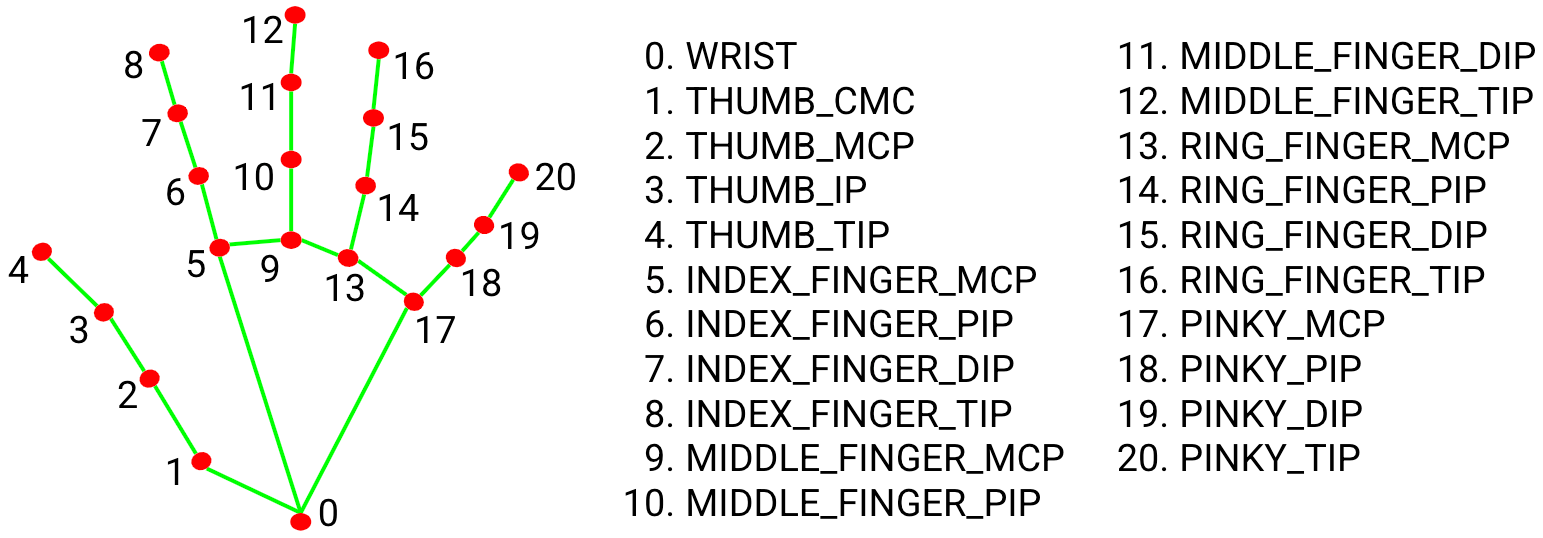
\includegraphics[width=\linewidth]{img/hand_landmarks} % Adjust the width or other parameters as needed
	\caption{Example of Hand Landmark obtained from Mediapipe}
	\label{fig:hand_landmark} % Reference the figure in your text using \ref{fig:unique_label}
\end{figure}

\section{Model architecture}
The model architecture for hand pose recognition typically combines convolutional neural networks (CNNs) for feature extraction with regression or classification layers for predicting hand poses. State-of-the-art models often utilize encoder-decoder frameworks to process input images and generate heatmaps or landmark coordinates. Mediapipe, for instance, uses a pipeline that first detects the hand region and then applies a specialized model to predict precise landmarks. Lightweight and efficient architectures are crucial to ensure real-time performance without compromising accuracy. These models are trained on large datasets to generalize across different hand shapes, orientations, and lighting conditions.

\section{Pose Estimation in 3D}
Pose estimation in 3D extends the capabilities of 2D models by incorporating depth information to reconstruct hand poses in a three-dimensional space. This process often integrates data from depth sensors or multi-view camera setups to triangulate landmark positions. 3D pose estimation provides more accurate representations of hand gestures, especially in scenarios involving rotations or occlusions. It is beneficial in applications like robotics, where precise hand positioning is required, or virtual reality, where realistic interactions with virtual objects depend on spatial accuracy. Each landmark consists of the following:
\begin{enumerate}
	\item $x$ and $y$: Landmark coordinates normalized to $[0.0, 1.0]$ by the image width and height respectively.
	\item $z$: Represents the landmark depth with the depth at the midpoint of hips being the origin, and the smaller the value the closer the landmark is to the camera. The magnitude of $z$ uses roughly the same scale as $x$.
	\item visibility: A value in $[0.0, 1.0]$ indicating the likelihood of the landmark being visible (present and not occluded) in the image.
\end{enumerate}




\section{Multi-Hand Support}
Multi-hand support is the capability of a hand pose recognition system to track and analyze multiple hands within the same frame simultaneously. This requires the model to distinguish between hands, assign unique identifiers, and accurately detect the landmarks for each hand. Challenges in multi-hand support include managing occlusions (where one hand partially covers the other) and handling varying hand orientations. Robust systems, like Mediapipe, employ efficient region segmentation and tracking algorithms to maintain consistent performance in multi-hand scenarios. Multi-hand support is essential for collaborative applications like multi-user gaming or shared virtual workspaces.